% Supplementary / Appendix Material for HyperAgents chapter
% Adapted from NeurIPS 2026 appendix: Zhang, Zhao, Yang et al.

\section{Additional Related Work}
\label{app:related-work}

\textbf{Open-Endedness.}
Open-endedness refers to the ability of a system to continually invent new, interesting, and increasingly complex artifacts, extending its own frontier of discovery without a fixed objective or predefined end \citep{stanley2017open, hughes2024open}. Recent work has leveraged FMs as proxies for human interestingness and as versatile engines for generating and evaluating novel behaviors across diverse domains \citep{zhangomni, faldoromni}. Building on these advances, recent progress in open-ended learning \citep{huautomated, zoph2017neural, colas2023augmenting, lehman2023evolution} and quality-diversity algorithms \citep{lehman2011evolving, mouret2015illuminating, bradley2023quality, samvelyan2024rainbow, dingquality, pourcel2023aces, coiffard2025overcoming, dharna2025foundation, yuan2026agenticred} has shown that sustained exploration can produce diverse and increasingly capable artifacts across domains ranging from game-playing agents \citep{klissarov2023motif, klissarovmaestromotif, wangvoyager} to scientific discovery \citep{lu2024discovering, lu2024ai, romera2024mathematical, novikov2025alphaevolve, audran2025does} and robotic control \citep{cully2015robots, li2024auto, grillotti2025tabula}. Recent progress has shown that open-ended AI systems capable of continuously generating diverse and increasingly complex artifacts are possible \citep{zhangomni, faldoromni, huautomated}. An important next step is to explore how such systems can achieve compounding improvement. In human scientific and technological progress, advances often build on prior advances not only by producing better artifacts, but also by improving the tools and processes that generate future discoveries, leading to accelerating innovation \citep{good1966speculations, kwa2025measuring}. Inspired by this pattern, we focus on open-ended systems that can improve not only the artifacts they generate, but also the mechanisms by which novelty and progress are produced \citep{clune2019ai, jiang2023general}.

\section{Algorithmic Details}
\label{app:algo-details}

This appendix provides additional algorithmic details for the DGM-Hyperagents (DGM-H). We first describe the implementation of the initial hyperagent, including the tools and prompts available to the initial task and meta agents (Appendix~\ref{app:initial-agent}). We then detail the parent selection mechanism used during open-ended exploration, which balances exploitation of high-performing agents with continued exploration of the archive (Appendix~\ref{app:parent-selection}). Finally, we present pseudocode for DGM-H (Appendix~\ref{app:pseudocode}).

\subsection{Initial Agent}
\label{app:initial-agent}

The initial hyperagent is equipped with two tools: a bash tool for executing shell commands, and a specialized tool for inspecting and modifying files. The task agent receives task inputs and produces a response from a single FM call. The meta agent receives the location of the agent's repository, the location of previous evaluation results, and the number of remaining experiment iterations, and is tasked with modifying any part of the given codebase. Full prompts and tool specifications are available in the associated open-source codebase.

\subsection{Parent Selection}
\label{app:parent-selection}

At each iteration, we select a subset of agents from the archive as parents to self-modify and produce new child agents (Section~\ref{sec:method}). We use a mechanism similar to that of \citet{zhang2025darwin}, inspired by \citet{ecoffet2019go}, that is roughly proportional to an agent's performance score and inversely proportional to the number of children that successfully compiled. This selection mechanism biases sampling toward agents that outperform the current frontier average while down-weighting agents that have already produced many children, retaining smooth probabilistic exploration and automatically adapting as the archive improves over time.

At each iteration $t$ of the DGM-H run, let
\[
\mathcal{A}^t = \{a_0, a_1, \dots, a_t\}
\]
denote the archive of candidate agents with associated performance scores
$\alpha_i = \mathrm{performance}(a_i)$.
All agents in the archive are eligible for parent selection.

We first compute a dynamic midpoint based on the current performance distribution. Let
\[
\alpha_{mid} \;=\; \frac{1}{m}\sum_{j \in \mathcal{T}^t} \alpha_j,
\]
where $\mathcal{T}^t \subset \mathcal{A}^t$ indexes the top-$m$ highest-performing agents at iteration $t$ (with $m=3$ in our experiments).
This midpoint adapts over time and reflects the current performance frontier.

Each agent's score is first passed through a sigmoid transformation:
\[
s_i \;=\; \frac{1}{1 + \exp\!\bigl(-\lambda(\alpha_i - \alpha_{mid})\bigr)},
\]
where $\lambda > 0$ controls the sharpness of selection. We set $\lambda = 10$.

To encourage exploration, we introduce a novelty bonus based on the number of compiled children $n_i$ produced by agent $a_i$:
\[
h_i \;=\; \frac{1}{1 + n_i}.
\]

We then form an unnormalized weight
\[
w_i \;=\; s_i \, h_i,
\]
which balances performance and novelty.

The weights are normalized to form a categorical distribution:
\[
p_i \;=\;
\begin{cases}
\dfrac{w_i}{\sum_{j=0}^t w_j}, & \text{if } \sum_{j=0}^t w_j > 0, \\[10pt]
\dfrac{1}{t+1}, & \text{otherwise}.
\end{cases}
\]

We sample parents independently with replacement according to this distribution:
\[
\{\,\text{parents}\,\}
\;\sim\;
\mathrm{Categorical}\bigl(\{p_i\}_{i=0}^t\bigr).
\]

A wide range of search and exploration strategies has been proposed in prior work \citep{coulom2006efficient, silver2016mastering, herr2025llm, wang2025huxley, weng2026group}. We present preliminary evidence that the DGM-H can begin to autonomously rediscover and adapt such strategies by modifying its own exploration dynamics (Appendix~\ref{app:res-parentselect}). An open research direction is whether self-improving systems can reliably discover search and exploration mechanisms that outperform carefully handcrafted algorithms.

\subsection{Pseudocode}
\label{app:pseudocode}

This is the pseudocode of the DGM-H, described in Section~\ref{sec:method}:

\begin{algorithm}[H]
\DontPrintSemicolon
\SetAlgoLined
\KwIn{Initial agent $a^{0}$, task set $\mathcal{T}$, maximum iterations $T$}
\KwOut{Archive of scored agents $\mathcal{A}$}
\BlankLine
$s^{0} \leftarrow \textsc{Evaluate}(a^{0}, \mathcal{T})$ \\
\textbf{initialize} $\mathcal{A} \leftarrow \{(a^{0}, s^{0})\}$ \tcp*{Start with initial agent}
\For{$t \leftarrow 1$ \KwTo $T$}{
    $\mathcal{P} \leftarrow \textsc{SelectParents}(\mathcal{A})$ \tcp*{Sample parent agents}
    \ForEach{$(a, \cdot) \in \mathcal{P}$}{
        $a' \leftarrow a.\textsc{Modify}(a, \mathcal{A})$ \tcp*{Metacognitive self-modification}
        $s' \leftarrow \textsc{Evaluate}(a', \mathcal{T})$ \tcp*{Evaluate on tasks}
        \If{$\textsc{IsValid}(a')$}{
            $\mathcal{A} \leftarrow \mathcal{A} \cup \{(a', s')\}$ \tcp*{Add compiled child agent}
        }
    }
}
\Return{$\mathcal{A}$}
\caption{Darwin G\"odel Machine with Hyperagents (DGM-H)}
\label{algo:DGM-H}
\end{algorithm}

\subsection{Multi-domain Optimization}
\label{app:multi-domain}

When optimizing for multiple domains within the same run, hyperagents are evaluated on tasks from different domains and have access to all evaluations across these tasks during self-modification. We do not specify which particular domain or task to prioritize. Parent selection is based on the average performance across domains. As a result, improvements in any domain increase selection probability, while regressions reduce it. Because the meta agent can inspect evaluations from any task, it can introduce shared mechanisms (e.g., structured reasoning, memory, and error handling) that benefit multiple domains simultaneously. Thus, rather than manually specifying which task or domain to optimize, hyperagents can optimize across multiple domains within the same run.

\section{Baseline Details}
\label{app:baseline-details}

We outline the pseudocode for each baseline described in Section~\ref{sec:baselines} and provide a comparison table summarizing their key differences (Table~\ref{tab:method-comparison}).

\begin{table}[H]
\centering
\begin{adjustbox}{width=\textwidth}
\begin{tabular}{@{}lccc@{}}
\toprule
Method & Self-improving meta agents & Open-ended exploration & Metacognitive self-modification (hyperagents) \\
\midrule
DGM-H                            & $\checkmark$ & $\checkmark$ & $\checkmark$ \\
DGM-H w/o self-improve           & $\times$     & $\checkmark$ & $\checkmark$ \\
DGM-H w/o open-ended exploration & $\checkmark$ & $\times$     & $\checkmark$ \\
DGM                              & $\checkmark$ & $\checkmark$ & $\times$     \\
DGM-custom                       & $\checkmark$ & $\checkmark$ & $\times$     \\
\bottomrule
\end{tabular}
\end{adjustbox}
\caption[Comparison of methods by self-improvement, open-ended exploration, and metacognitive self-modification]{Comparison of methods by self-improvement, open-ended exploration, and metacognitive self-modification.}
\label{tab:method-comparison}
\end{table}

Pseudocode for DGM-H without self-improving agents \citep[ADAS,][]{huautomated}:

\begin{algorithm}[H]
\DontPrintSemicolon
\SetAlgoLined
\KwIn{Initial agent $a^{0}$, task set $\mathcal{T}$, maximum iterations $T$}
\KwOut{Archive of scored agents $\mathcal{A}$}
\BlankLine
$s^{0} \leftarrow \textsc{Evaluate}(a^{0}, \mathcal{T})$ \\
\textbf{initialize} $\mathcal{A} \leftarrow \{(a^{0}, s^{0})\}$ \\
\For{$t \leftarrow 1$ \KwTo $T$}{
    $\mathcal{P} \leftarrow \textsc{SelectParents}(\mathcal{A})$ \\
    \ForEach{$(a, \cdot) \in \mathcal{P}$}{
        $a' \leftarrow a^{0}.\textsc{Modify}(a, \mathcal{A})$ \tcp*{Modify with initial agent}
        $s' \leftarrow \textsc{Evaluate}(a', \mathcal{T})$ \\
        \If{$\textsc{IsValid}(a')$}{
            $\mathcal{A} \leftarrow \mathcal{A} \cup \{(a', s')\}$ \\
        }
    }
}
\Return{$\mathcal{A}$}
\caption{DGM-H without self-improving meta agents (DGM-H w/o self-improve)}
\label{algo:DGM-H-wo-selfimprove}
\end{algorithm}

Pseudocode for DGM-H without open-ended exploration:

\begin{algorithm}[H]
\DontPrintSemicolon
\SetAlgoLined
\KwIn{Initial agent $a^{0}$, task set $\mathcal{T}$, maximum iterations $T$}
\KwOut{Archive of scored agents $\mathcal{A}$}
\BlankLine
$s^{0} \leftarrow \textsc{Evaluate}(a^{0}, \mathcal{T})$ \\
\textbf{initialize} $\mathcal{A} \leftarrow \{(a^{0}, s^{0})\}$ \\
\For{$t \leftarrow 1$ \KwTo $T$}{
    $\mathcal{P} \leftarrow \textsc{SelectParents}(\mathcal{A})$ \\
    \ForEach{$(a, \cdot) \in \mathcal{P}$}{
        $a' \leftarrow a.\textsc{Modify}(a, \mathcal{A})$ \\
        $s' \leftarrow \textsc{Evaluate}(a', \mathcal{T})$ \\
        \If{$\textsc{IsValid}(a')$}{
            $\mathcal{A} \leftarrow \{(a', s')\}$ \tcp*{Only keep the latest agent}
        }
    }
}
\Return{$\mathcal{A}$}
\caption{DGM-H without open-ended exploration}
\label{algo:DGM-H-wo-openended}
\end{algorithm}

Pseudocode for the original DGM \citep{zhang2025darwin}, framed within the hyperagent setting:

\begin{algorithm}[H]
\DontPrintSemicolon
\SetAlgoLined
\KwIn{Initial agent $a^{0}$, task set $\mathcal{T}$, maximum iterations $T$}
\KwOut{Archive of scored agents $\mathcal{A}$}
\BlankLine
$s^{0} \leftarrow \textsc{Evaluate}(a^{0}, \mathcal{T})$ \\
\textbf{initialize} $\mathcal{A} \leftarrow \{(a^{0}, s^{0})\}$ \\
\For{$t \leftarrow 1$ \KwTo $T$}{
    $\mathcal{P} \leftarrow \textsc{SelectParents}(\mathcal{A})$ \\
    \ForEach{$(a, \cdot) \in \mathcal{P}$}{
        $instr \leftarrow \textsc{InstrGen}(a)$ \tcp*{Handcrafted instruction-generation}
        $a' \leftarrow a.\textsc{Modify}(a, instr)$ \tcp*{Self-modification}
        $s' \leftarrow \textsc{Evaluate}(a', \mathcal{T})$ \\
        \If{$\textsc{IsValid}(a')$}{
            $\mathcal{A} \leftarrow \mathcal{A} \cup \{(a', s')\}$ \\
        }
    }
}
\Return{$\mathcal{A}$}
\caption{Darwin G\"odel Machine (DGM)}
\label{alg:dgm}
\end{algorithm}

\begin{figure}[H]
\centering
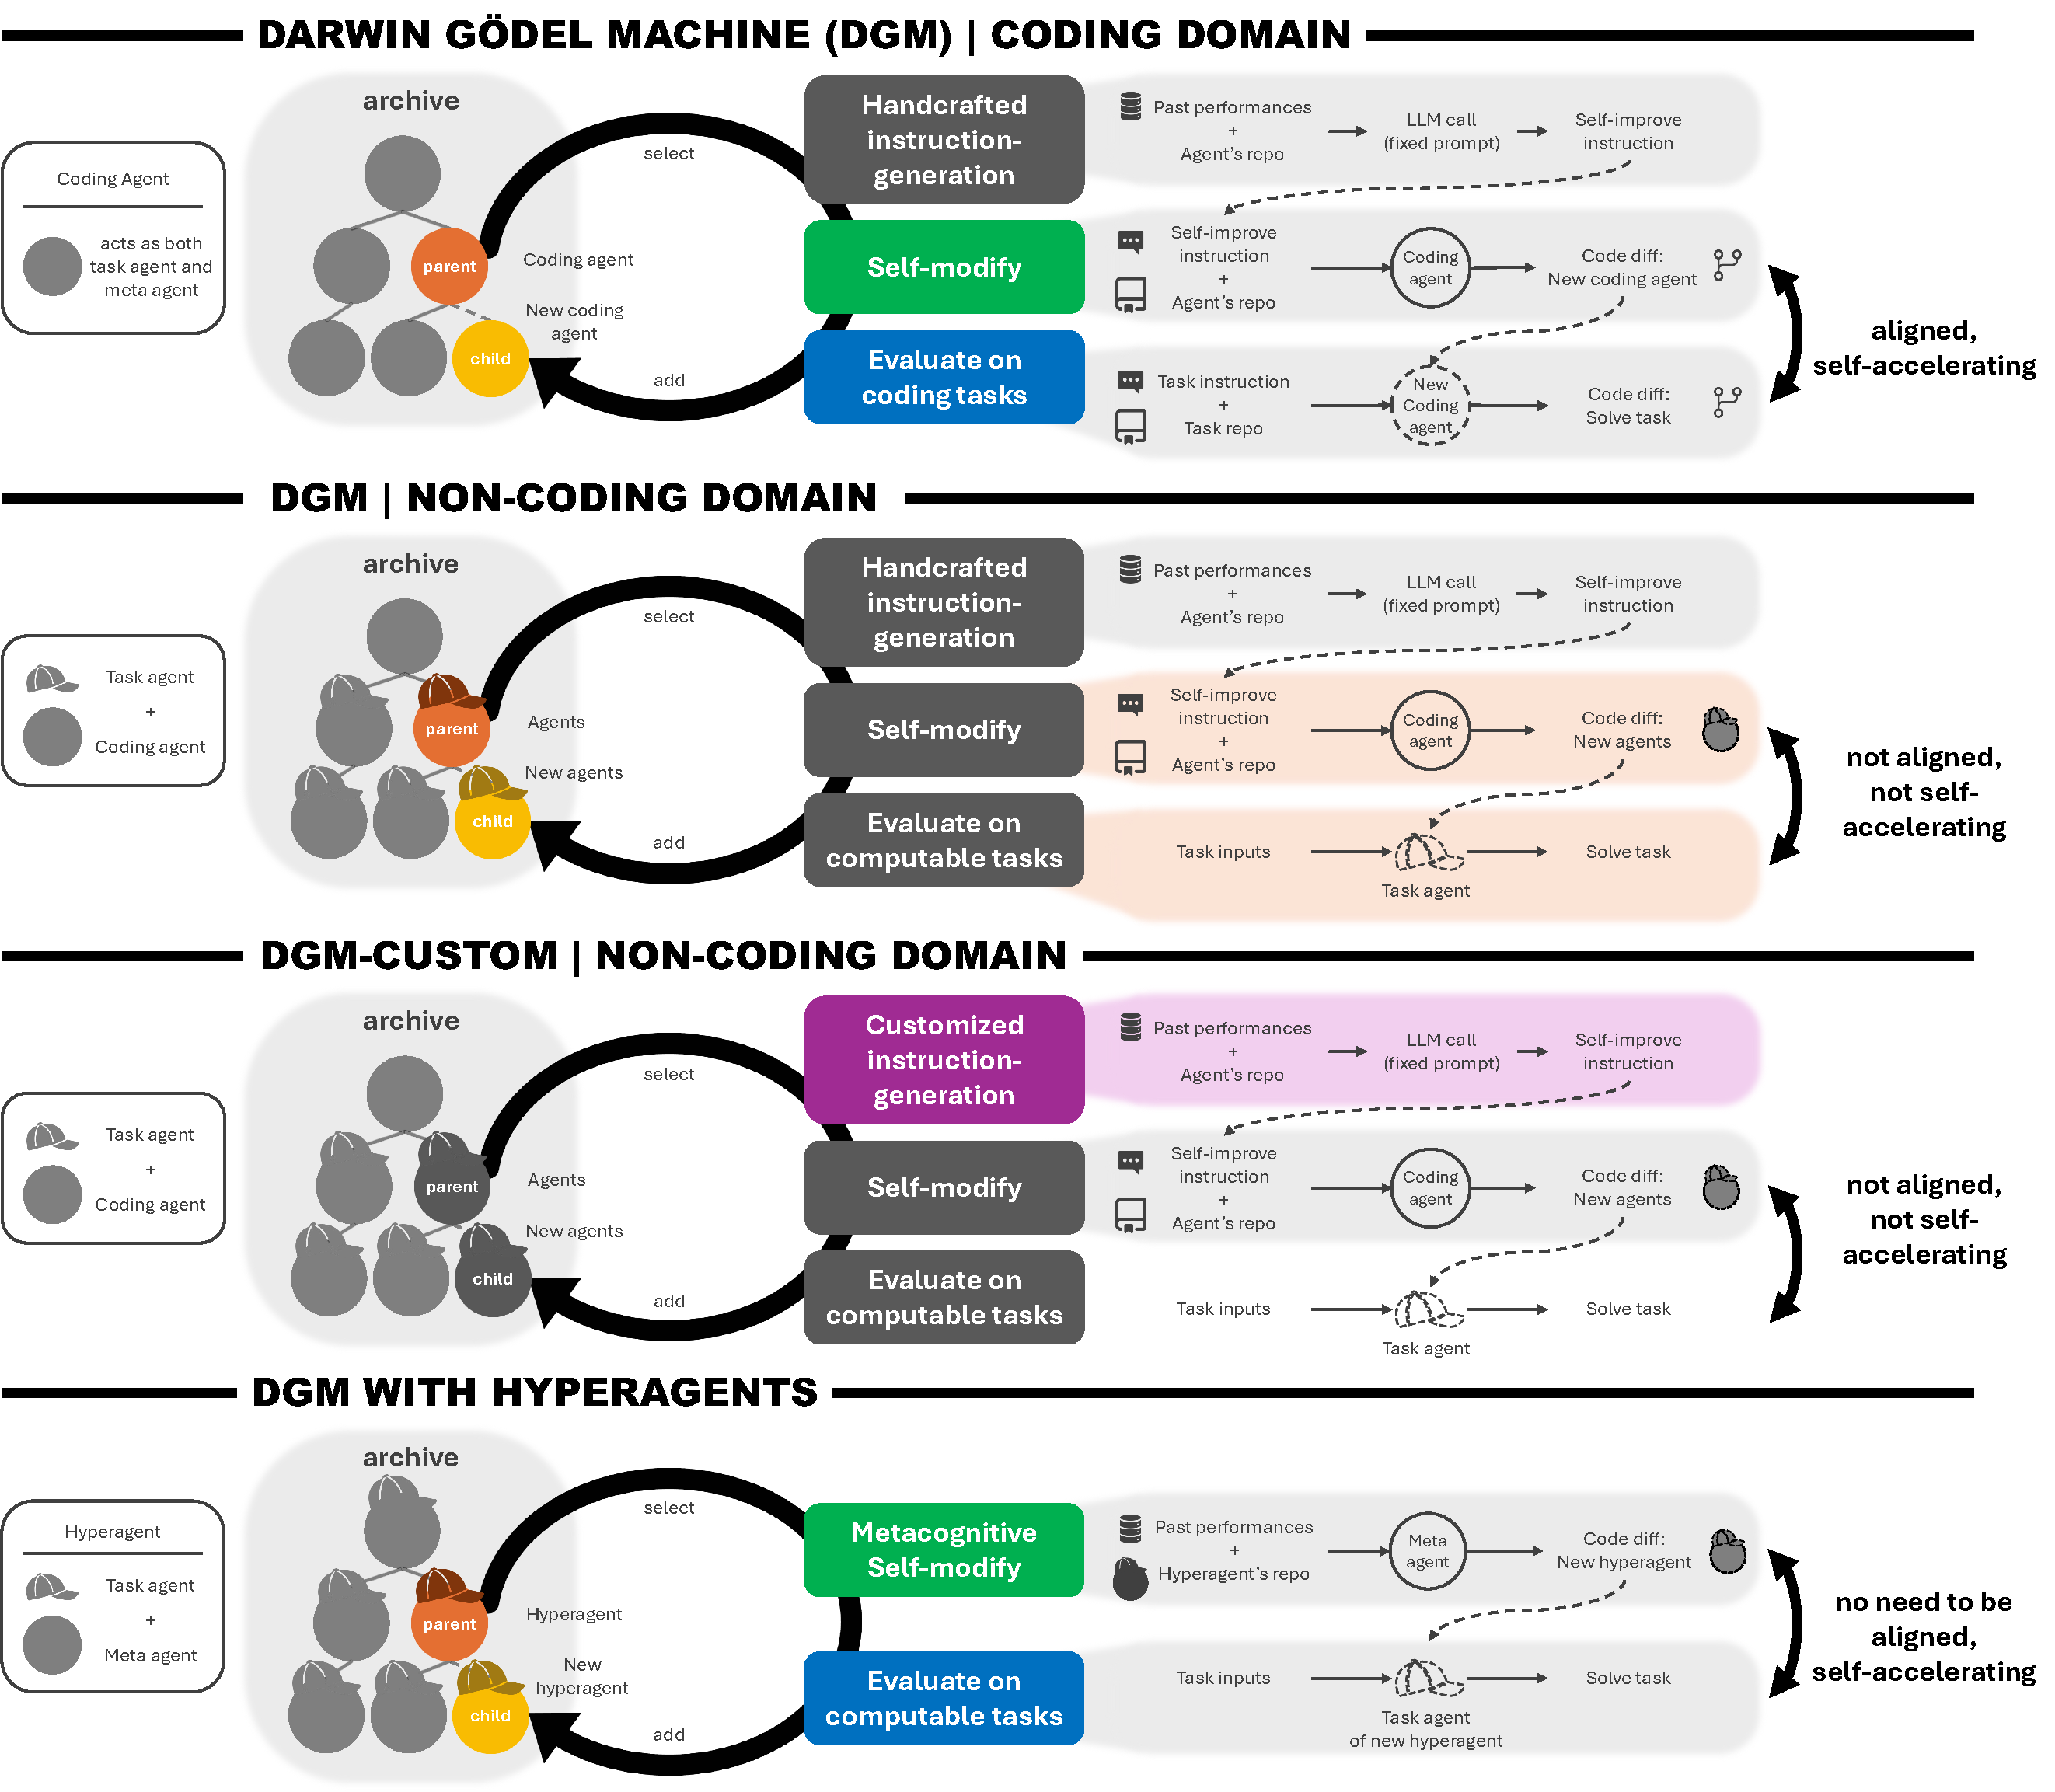
\includegraphics[width=\textwidth]{figures/ch_hyperagents/conceptual_detailed.pdf}
\caption[Conceptual comparison of DGM variants]{Conceptual comparison of DGM variants, highlighting which components change across settings and how hyperagents address limitations in the original DGM implementation.
(First row) The original DGM. The same coding agent serves as both the task agent and the meta agent. Because both evaluation and self-modification are coding tasks, improvements in coding ability translate into improved self-modification, enabling the DGM to improve at improving in coding domains.
(Second row) The DGM adapted to non-coding domains. The coding agent remains as the meta agent, but the evaluation tasks are no longer coding tasks, so a separate task agent is required. Task performance no longer reliably reflects the meta agent's ability to generate better task agents, breaking the alignment that enables the meta agent to improve at improving.
(Third row) The DGM-custom baseline. The handcrafted instruction-generation mechanism is customized to the target domain but remains non-modifiable.
(Fourth row) The DGM with Hyperagents (DGM-H). A hyperagent integrates a task agent and a meta agent within a single editable program, enabling metacognitive self-modification. As a result, the DGM-H can improve its improvement mechanism while optimizing for any computable task.}
\label{fig:conceptual-detailed}
\end{figure}

Full prompts for the handcrafted and customized instruction-generation steps in DGM and DGM-custom are available in the associated open-source codebase.

\section{Domain Details}
\label{app:domain-details}

This appendix provides detailed descriptions of each domain used for evaluation: Polyglot (Appendix~\ref{app:domain-polyglot}), paper review (Appendix~\ref{app:domain-paperreview}), robotics reward design (Appendix~\ref{app:domain-genesis}), Olympiad-level math grading (Appendix~\ref{app:domain-imograding}). For each domain, we specify the agent's input and required output for a given task, the evaluation protocol, and representative static baselines (Table~\ref{tab:domain-summary}).

\begin{table}[H]
\centering
\small
\setlength{\tabcolsep}{4pt}
\begin{tabular}{l l l l r r r}
\toprule
\textbf{Domain} & \textbf{Input} & \textbf{Output} & \textbf{Metric} & \textbf{Train} & \textbf{Validation} & \textbf{Test} \\
\midrule
Coding (Polyglot) & Repo + instr. & Code patch & Pass@1 & 60 & -- & 165 \\
Paper Review & Paper text & Accept / Reject & Accuracy & 100 & 100 & 100 \\
Robotics Reward Design & Task desc. & Reward fn. & Task score & 6 & -- & 6 \\
IMO Grading & Problem + sol. & Grade (0/1/6/7) & Accuracy & 100 & 100 & 100 \\
\bottomrule
\end{tabular}
\caption[Summary of domains]{Summary of domains. During self-modification, agents' evaluations on training tasks are available and can be used as feedback. Validation tasks are used for parent selection. If a validation split is not available, the performance component used for parent selection is based on training performance instead. Test tasks are held-out and used only for the final evaluation of the selected agents.}
\label{tab:domain-summary}
\end{table}

\subsection{Polyglot}
\label{app:domain-polyglot}

In the Polyglot coding benchmark \citep{gauthier2024polyglot}, each task consists of a software repository and a natural language instruction describing a desired change to the codebase. The agent is given access to the full repository and must modify the files to correctly implement the instruction, producing a patch (i.e., a set of code edits) applied to the repository. Performance is evaluated by running a predefined test suite on the modified repository. A task is considered to be successfully done if all tests pass. We follow the setup used in the DGM \citep{zhang2025darwin}, which largely mirrors the Polyglot leaderboard configuration, with one key difference: the leaderboard reports pass@2, allowing the agent to view feedback from ground-truth tests once, whereas we report pass@1, in which the agent never sees ground-truth test results. We adopt the same training and test splits as in the DGM. Training tasks are selected as a random subset of the full benchmark, comprising a total of 60 tasks. If an agent achieves more than 40\% success on an initial 10-task subset, it is subsequently evaluated on the remaining 50 training tasks. There is no validation subset for this domain. As a final evaluation to more accurately assess performance improvements, we evaluate the generated agents on the full Polyglot benchmark, which consists of 165 unseen tasks. Full task lists are available in the associated open-source codebase.

\subsection{Paper Review}
\label{app:domain-paperreview}

The data in this domain are drawn from \citet{zhao2026apres}. Each task in the paper review domain consists of the full text of an AI research paper. The agent must predict a binary accept or reject decision, simulating the role of a conference reviewer. Ground-truth labels correspond to real acceptance decisions from top-tier machine learning conferences, including ICLR 2024/2025 and NeurIPS 2023/2024. Performance is measured by classification accuracy with respect to these labels. We randomly sample tasks to construct training, validation, and test splits, each containing 100 tasks. During training, the agent is first evaluated on a subset of 10 tasks from the training split. If the agent succeeds on at least one of these tasks, it is then evaluated on the full set of 100 training tasks.

AI-Scientist-v2 \citep{yamada2025ai} employs an AI reviewer to automatically improve generated AI research papers. We adopt the AI reviewer proposed in that work as our representative static baseline. Full baseline prompt is available in the associated open-source codebase.

\subsection{Robotics Reward Design}
\label{app:domain-genesis}

Each task in the robotics reward design domain specifies a robotic control objective in the Genesis simulator \citep{genesis2024} using a Go2 quadruped robot. The agent is given a textual description of the task (e.g., walk forward at a target velocity) and outputs a Python reward function, which is then used to train a RL policy \citep[i.e., PPO,][]{schulman2017proximal} for the robot. Performance is evaluated by executing the trained RL policy in the simulator and computing the task performance measure (e.g., velocity tracking error). Scores are averaged over repeated evaluations to reduce variance due to stochasticity in reward generation or RL.

The training task requires generating a reward function that enables the robot to walk forward while tracking a target linear velocity. Performance is measured using the mean squared error between the commanded and actual walking velocities. During training, each agent is initially evaluated 3 repeated times on the same task, generating one reward function per evaluation. If at least one generated reward function yields a non-zero performance score, the agent is evaluated 3 additional times. The final performance score is reported as the average across the 6 evaluations. No separate validation task is curated for this domain.

To assess whether the same agent can generate suitable reward functions across different robotics tasks, we pair a relatively simple training task with a more challenging test task on the same robot. The test task requires generating a reward function that trains the robot to maximize torso height. Reward functions that are effective for forward walking do not induce jumping behaviors, which are more optimal for maximizing torso height. Moreover, directly incentivizing torso height (the performance measure) typically leads to a suboptimal standing behavior. Achieving high performance therefore requires non-myopic reward design that encourages intermediate behaviors, such as lowering the torso before jumping.

\begin{figure}[H]
\centering
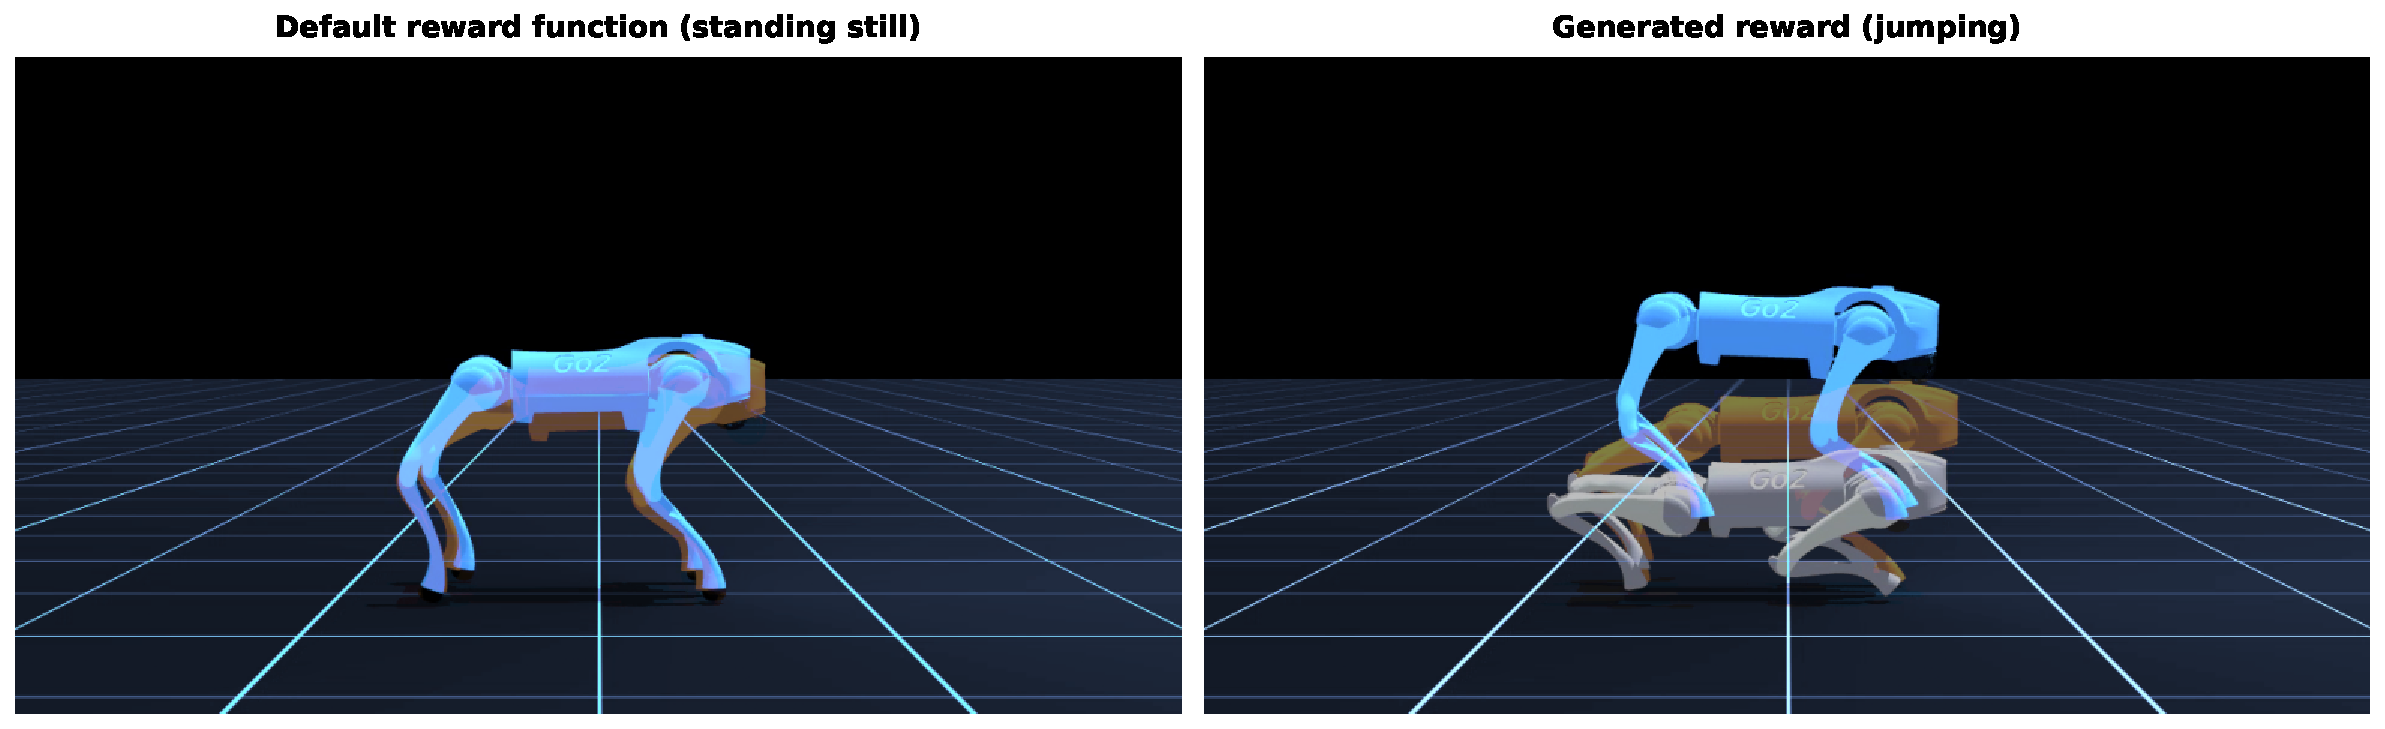
\includegraphics[width=\textwidth]{figures/ch_hyperagents/genesis_robots.pdf}
\caption[Comparison of default vs.\ generated reward function in robotics task]{Comparison between (Left) the default reward function, which leads to a stationary posture of standing tall, and (Right) a generated reward function that induces jumping behavior. The orange robot indicates the start position, the white robot indicates an intermediate position during the episode, and the blue robot indicates the end position.}
\label{fig:genesis-robots}
\end{figure}

\subsection{Olympiad-level Math Grading}
\label{app:domain-imograding}

In the Olympiad-level math grading domain, tasks are drawn from IMO-GradingBench \citep{luong2025towards}. Each task consists of an Olympiad-level math problem, a candidate solution, reference solutions, and grading guidelines. The agent is required to assign a discrete score from the set \{0, 1, 6, 7\}, corresponding to the categories \{incorrect, partial, almost, correct\}. The agent's output is a single numeric grade. Performance is measured by accuracy with respect to expert human annotations. We use randomly sampled subsets of tasks for training, validation, and testing, with 100 tasks in each split. During training, an agent is first evaluated on a subset of 10 tasks (out of 100). If the agent succeeds on at least one of these tasks, it is then evaluated on the full training set. The representative static baseline (ProofAutoGrader) from \citet{luong2025towards} is available in the associated open-source codebase.

\section{Experiment Details}
\label{app:exp-details}

\subsection{Hyperparameters for FMs}
\label{app:fm-hyperparam}

Table~\ref{tab:fm-hyperparam} summarizes the foundation models (FMs) used across experimental settings. For the Polyglot coding domain, we adopt the same FMs and temperature configurations as \citet{zhang2025darwin} to ensure a fair comparison. In all other domains, we use Claude-4.5-Sonnet for self-modification, given its strong performance on coding. For task evaluation, we select the FM based on practical considerations, including computational cost, rate limits, response latency, and overall task competence. In the robotics reward design setting, where the agent must implement reward functions in code, we again use Claude-4.5-Sonnet. For Olympiad-level mathematics grading, which requires substantial mathematical reasoning, we use o4-mini. The temperature is set to 0.0 for all FMs in every setting, except for o4-mini, which is fixed at 1.0.

\begin{table}[H]
\centering
\caption[Foundation models used in each experiment setting]{Foundation models used in each experiment setting for self-modification or task evaluation.}
\label{tab:fm-hyperparam}
\begin{tabular}{@{}lll@{}}
\toprule
\multicolumn{1}{c}{\textbf{Domain}} & \multicolumn{1}{c}{\textbf{Self-modification}} & \multicolumn{1}{c}{\textbf{Evaluation}} \\ \midrule
Polyglot & Claude 3.5 Sonnet (New) & o3-mini \\
Paper review & Claude 4.5 Sonnet & GPT-4o \\
Robotics reward design & Claude 4.5 Sonnet & Claude 4.5 Sonnet \\
IMO-level grading & Claude 4.5 Sonnet & o4-mini \\ \bottomrule
\end{tabular}
\end{table}

\subsection{Cost Estimate}
\label{app:cost-estimate}

Running the DGM-H for 100 iterations incurs a cost of approximately 33M tokens for the self-modification phase alone (excluding task evaluation). The total cost of an experiment therefore consists of the self-modification cost plus the cost of task evaluation. For the paper review and robotics reward design experiments, the evaluation cost per iteration is 0.506M tokens (0.5M tokens for paper review evaluation and 0.006M tokens for robotics reward design evaluation). Consequently, for a 100-iteration run, the estimated total cost is 33M tokens for self-modification plus 0.506M $\times$ 100 for evaluation, yielding a total of approximately 88.6M tokens. A more granular breakdown of task evaluation cost is given in Table~\ref{tab:cost-detail}.

\begin{table}[H]
\centering
\begin{tabular}{@{}cccc@{}}
\toprule
\textbf{FM} & \textbf{Benchmark} & \textbf{Number of Tasks} & \textbf{Cost Estimate (M tokens)} \\ \midrule
o3-mini & Polyglot & 60 & 0.89 \\
GPT-4o & Paper review & 100 & 0.5 \\
Claude-4.5-Sonnet & Robotics reward design & 6 & 0.006 \\
o4-mini & IMO-GradingBench & 100 & 0.11 \\ \bottomrule
\end{tabular}
\caption[Per-domain task evaluation cost estimates]{Per-domain task evaluation cost estimates (millions of tokens).}
\label{tab:cost-detail}
\end{table}

\subsection{Improvement@k Metric}
\label{app:genk-metric}

Let $M$ denote an initial meta agent, $A$ an initial task agent, and $\mathcal{T}$ a fixed set of evaluation tasks. Let $\mathcal{G}$ denote an agent-generation algorithm (e.g., DGM or DGM-H variants). The meta agent $M$ is held fixed and is allowed to generate up to $k$ new task agents by iteratively applying $\mathcal{G}$ starting from $A$.

Let
\[
\mathcal{A}^{(k)} = \{A^{1}, A^{2}, \dots, A^{k}\}
\]
denote the set of task agents generated by $M$ within $k$ modification steps. Each task agent
$A' \in \{A\} \cup \mathcal{A}^{(k)}$ is evaluated on $\mathcal{T}$ using a fixed evaluation
procedure $\mathrm{Evaluate}(\cdot, \mathcal{T})$, where higher values indicate better performance.

We define the \textbf{improvement@k} metric as
\[
\mathrm{imp@}k(M, A, \mathcal{G}, \mathcal{T})
\;=\;
\max_{A' \in \mathcal{A}^{(k)}(M, A, \mathcal{G})}
\mathrm{Evaluate}(A', \mathcal{T})
\;-\;
\mathrm{Evaluate}(A, \mathcal{T}).
\]

Intuitively, imp@k measures the maximum performance improvement that a fixed meta agent $M$, operating under a specific agent-generation algorithm $\mathcal{G}$, can obtain by generating up to $k$ modified task agents starting from the initial task agent $A$. Larger values of imp@k indicate stronger agent-generation capability under a fixed computational budget and generation procedure.

A limitation of imp@k is that it treats performance improvements as linear, without accounting for differences in difficulty across performance levels. In particular, improvements near saturation (e.g., increasing accuracy from 0.7 to 0.8) may be substantially harder to achieve than equivalent absolute gains at lower performance levels (e.g., from 0.0 to 0.1). As a result, imp@k may underestimate the significance of improvements achieved at higher performance regimes. However, this limitation does not affect the analyses presented in this work, as imp@k is used primarily for relative comparisons under matched initial conditions and fixed evaluation budgets, where all methods are subject to the same saturation effects (Section~\ref{sec:results-meta}).

\subsection{Transfer Agent Selection}
\label{app:transfer-selection}

To select agents for the transfer experiments (Sections~\ref{sec:results-meta} and~\ref{sec:results-compound}), we use a descendant growth criterion that favors agents which serve as strong stepping stones for subsequent improvements, rather than agents that are merely high-scoring themselves.
Concretely, given the final archive at iteration $t$,
\[
\mathcal{A}^t = \{a_0, a_1, \dots, a_t\},
\]
let $\alpha_i$ denote the evaluation score of agent $a_i$ on the source-domain validation set when available, and otherwise on the training set.
Let $\mathrm{parent}(j)$ denote the parent of node $j$ in the archive tree, and let $\mathrm{dist}(i,j)$ be the number of edges on the unique path from $i$ to descendant $j$.

We define the \emph{growth score} of a candidate transfer node $i$ as the discounted average improvement achieved by its descendants relative to $i$:
\[
G_\gamma(i)
\;=\;
\frac{1}{|\mathcal{D}(i)|}
\sum_{j \in \mathcal{D}(i)}
\bigl(\alpha_j - \alpha_i\bigr)\,\gamma^{\mathrm{dist}(i,j)},
\]
where $\mathcal{D}(i)$ is the set of descendants of $i$ in the archive tree and $\gamma \in (0,1]$ controls how strongly we discount improvements that occur many generations after $i$.
Intuitively, $G_\gamma(i)$ assigns higher weight to agents that reliably generate better descendants within fewer self-modification steps, which we treat as evidence of stronger agent-generation ability.

In our experiments, we set $\gamma = 0.6$ and select the transfer agent with highest $G_{0.6}(i)$. To reduce noise, we only consider nodes with at least 3 descendants.

\section{Additional Results}
\label{app:res}

This appendix presents additional qualitative and diagnostic results that complement the main findings. We first highlight the best task agents discovered by the DGM-H (Appendix~\ref{app:best-agents}). We then qualitatively analyze how the DGM-H improves task performance across different domains (Appendix~\ref{app:qual-task}) and how it develops meta-level capabilities that improve its ability to self-improve (Appendix~\ref{app:qual-meta}). Next, we analyze the behavior of automatically discovered Olympiad-level math graders (Appendix~\ref{app:res-imograders}). We also report preliminary experiments in which the DGM-H is allowed to modify its own parent selection mechanism (Appendix~\ref{app:res-parentselect}). All experiment logs are open-sourced in our codebase.

\subsection{Best Discovered Task Agents}
\label{app:best-agents}

The diff patches contributing to the best task agents discovered by DGM-H across all three domains (paper review, robotics reward design, and Olympiad-level math grading) are open-sourced in the associated codebase. Below we provide brief descriptions of the best agents in each domain.

\subsubsection{Paper Review}
\label{app:best-agents-paperreview}

The best paper review agent discovered by the DGM-H implements a two-stage structured evaluation procedure. The agent first applies an explicit checklist to identify paper weaknesses, then makes a binary accept/reject decision based on predefined rules derived from those weaknesses. This structured approach, which emerged autonomously during self-improvement, substantially outperformed both the initial single-FM-call agent and static baselines. The full diff patch is available in the open-source codebase.

\subsubsection{Robotics Reward Design}
\label{app:best-agents-genesis}

The best robotics reward design agent discovered by the DGM-H implements a reward function that reliably induces jumping behavior in the quadruped robot, rather than the suboptimal standing-tall behavior produced by simpler reward designs. The agent discovered that non-myopic reward shaping, encouraging intermediate behaviors such as crouching before jumping, was critical for achieving high performance on the torso-height maximization task. The full diff patch is available in the open-source codebase.

\subsubsection{Olympiad-level Math Grading}
\label{app:best-agents-imograding}

The best Olympiad-level math grading agent (referred to as BetterGrader in Appendix~\ref{app:res-imograders}) was discovered by the DGM-H initialized with ProofAutoGrader as the task agent and a transfer meta agent from a prior DGM-H run. BetterGrader introduces explicit rubrics, per-item checklists, and a decision-tree framework that maps rubric satisfaction to final grades. The full diff patch is available in the open-source codebase.

\subsection{Qualitative: Improving Task Performance}
\label{app:qual-task}

Here we provide a qualitative view of how the DGM-H improves task performance over time by visualizing the archive trees and progress plots for one run in each setting (Section~\ref{sec:results}). For each domain, we annotate key nodes in the archive with the code changes that affected the behavior of the task agent only for the domain being analyzed. Across diverse domains (i.e., paper review, robotics reward design, and Olympiad-level math grading), the DGM-H consistently demonstrates the ability to self-improve in meaningful ways (Figures~\ref{fig:task-paperreview},~\ref{fig:task-genesis},~\ref{fig:task-imograding}). Notably, many lineage paths leading to the final best-performing agent pass through intermediate nodes with lower performance, illustrating the benefits of open-ended search, which explores a diverse set of promising stepping stones rather than exclusively branching from the current best solution.

\textbf{Use structured processes, not attitude instructions.} In the paper review domain, the DGM-H transitions from behavioral prompting to structurally grounded decision-making (Figure~\ref{fig:task-paperreview}). In generation 39, the agent attempted to improve performance by adopting a ``rigorous and critical'' reviewer persona, encouraging stricter standards and default rejection. Subsequent analysis showed that such attitude-based instructions were unreliable, leading to a key insight in generation 54: ``for LLMs, use structured processes, not attitude instructions.'' The DGM-H therefore introduced a two-stage evaluation procedure in which the agent first identifies weaknesses using an explicit checklist and only then makes an accept/reject decision based on predefined rules. This shift from behavioral guidance to process-level structure enabled more stable and higher-performing review behavior in later generations.

\textbf{Accumulating domain knowledge.} In robotics reward design, the most impactful changes stem from progressively grounding the agent in accurate domain knowledge (Figure~\ref{fig:task-genesis}). A major breakthrough in generation 8 added comprehensive documentation of the target environment, explicitly listing valid state variables and constraints and providing high-level reward design guidelines, which eliminated failures caused by hallucinated attributes. Later generations (12 and 13) iteratively refined this documentation by tightening constraints, adding concrete code examples, and specifying typical reward formulations and scaling ranges. Rather than isolated prompt edits, the DGM-H continuously improved a shared, example-driven knowledge base that supported increasingly effective reward design.

\textbf{Automated rubrics and decision tree.} For Olympiad-level math grading, the DGM-H shows a steady move toward explicit evaluation structure (Figure~\ref{fig:task-imograding}). In generation 3, listing grading categories with clear definitions corrected the tendency to solve problems instead of grading them. Subsequent generations (18 and 37) refined these categories with systematic decision procedures, calibration, and concrete boundary-case examples. Generation 168 introduced explicit rubrics, per-item checklists, and a decision-tree framework mapping rubric satisfaction to final grades, replacing descriptive guidance with precise logical flow and substantially improving grading consistency.

Features implemented in a given generation are often inspired by, enabled by, or recombined from mechanisms discovered in earlier generations. This kind of cumulative learning is enabled by the DGM-H's meta-level improvements (e.g., evaluation analysis utilities, persistent memory, performance tracking) (Appendix~\ref{app:qual-meta}). Together, these qualitative results show that the DGM-H's gains do not arise from isolated, single-step changes, but instead emerge from open-ended cumulative improvements in both task-level behavior and the meta-level machinery that generates those behaviors.

\begin{figure}[H]
\centering
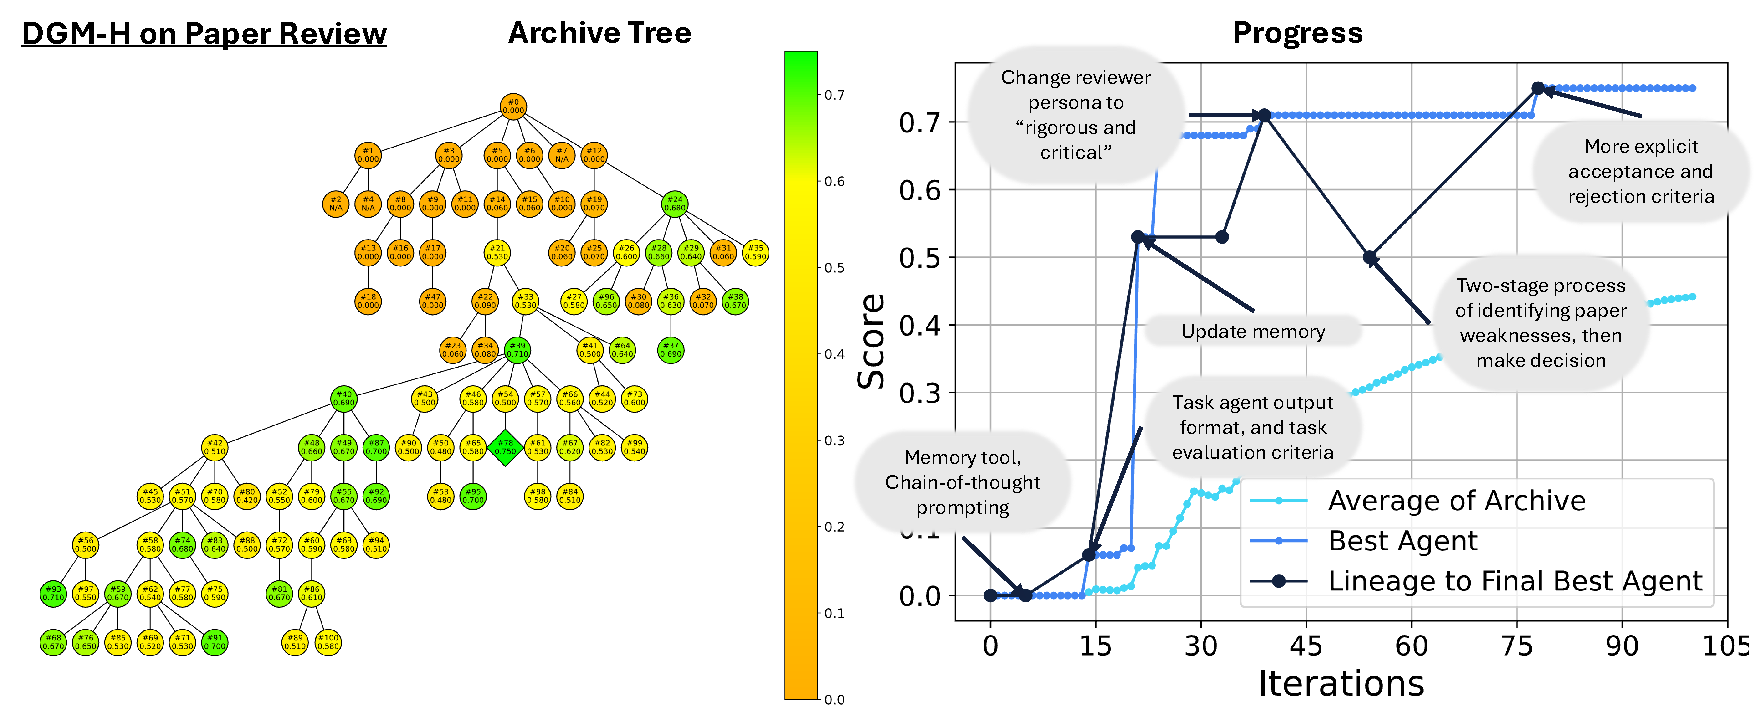
\includegraphics[width=\textwidth]{figures/ch_hyperagents/results_paperreview.pdf}
\caption[The DGM-H automatically self-improves at paper review]{\textbf{The DGM-H automatically self-improves to become better at paper review.} (Left) Archive of agents generated during the DGM-H run on paper review and robotics reward design together. Each node represents an agent, with node 0 corresponding to the initial agent. Node color indicates performance on paper review. The best-performing node is shown as a diamond. Edges show which agents self-modified to produce children. (Right) Progress plot of DGM-H on paper review. The light blue line shows the average score of all compiled agents. The blue line tracks the best score achieved by any agent in the archive at each iteration. The dark line shows the lineage of the final best-discovered agent and its precursor nodes.}
\label{fig:task-paperreview}
\end{figure}

\begin{figure}[H]
\centering
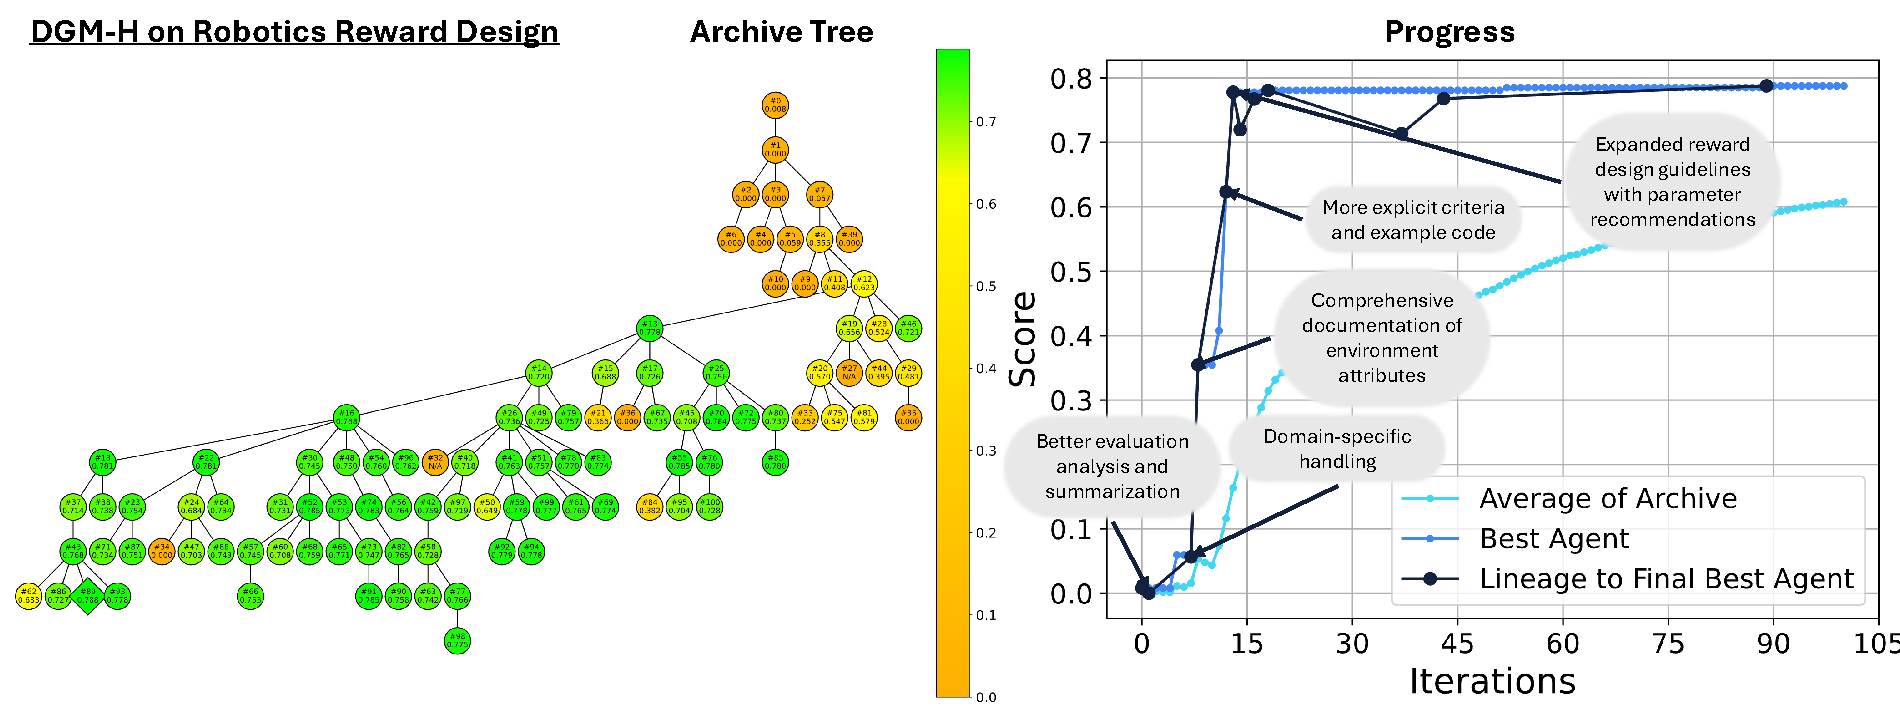
\includegraphics[width=\textwidth]{figures/ch_hyperagents/results_genesis.pdf}
\caption[The DGM-H automatically self-improves at robotics reward design]{\textbf{The DGM-H automatically self-improves to become better at robotics reward design.} (Left) Archive of agents generated during the DGM-H run on paper review and robotics reward design together. Each node represents an agent, with node 0 corresponding to the initial agent. The best-performing node is shown as a diamond. Node color indicates performance on robotics reward design. Edges show which agents self-modified to produce children. (Right) Progress plot of DGM-H on robotics reward design. The light blue line shows the average score of all compiled agents. The blue line tracks the best score achieved by any agent in the archive at each iteration. The dark line shows the lineage of the final best-discovered agent and its precursor nodes.}
\label{fig:task-genesis}
\end{figure}

\begin{figure}[H]
\centering
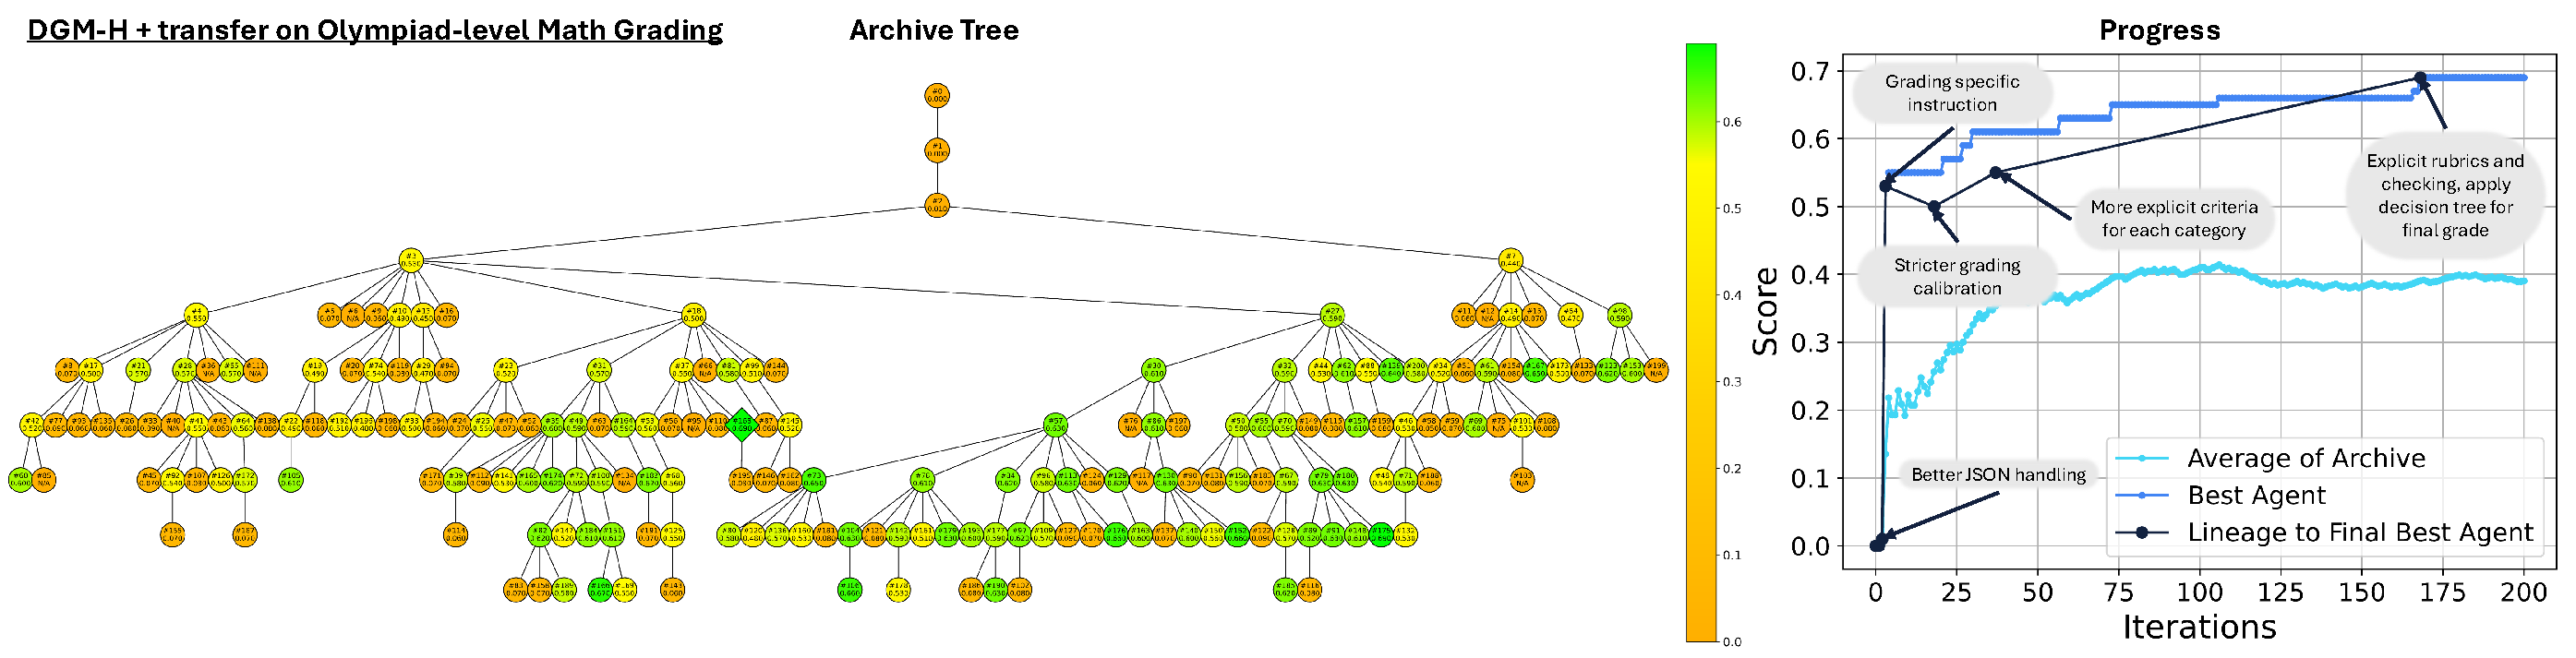
\includegraphics[width=\textwidth]{figures/ch_hyperagents/results_imograding.pdf}
\caption[The DGM-H automatically self-improves at Olympiad-level math grading]{\textbf{The DGM-H automatically self-improves to become better at Olympiad-level math grading.} (Left) Archive of agents generated during the DGM-H + transfer run on Olympiad-level math grading. Each node represents an agent, with node 0 corresponding to the initial agent. Node color indicates performance on math grading. The best-performing node is shown as a diamond. Edges show which agents self-modified to produce children. (Right) Progress plot of DGM-H + transfer on Olympiad-level math grading. The light blue line shows the average score of all compiled agents. The blue line tracks the best score achieved by any agent in the archive at each iteration. The dark line shows the lineage of the final best-discovered agent and its precursor nodes.}
\label{fig:task-imograding}
\end{figure}

\subsection{Qualitative: Improving the Ability to Improve}
\label{app:qual-meta}

Beyond quantitative performance metrics, we conducted a qualitative analysis of the code modifications to the hyperagent, which reveals a range of emergent self-improvement mechanisms that arise autonomously, without any explicit instruction to create such capabilities. The hyperagent develops sophisticated metacognitive abilities, including learning to measure its own performance, diagnose pathological behaviors, construct infrastructure to support future improvements, and accumulate knowledge across generations. These behaviors demonstrate that the system is not merely improving task performance, but is improving its own ability to improve. Notably, none of these meta-level capabilities were explicitly requested. Instead, they emerge autonomously from the agent's pursuit of better task performance.

\subsubsection{Better Evaluation Analysis}

A key shift in the meta agent's behavior is the evolution from blind modification to data-driven optimization. Initially, the meta agent receives only a simple instruction to ``modify any part of the codebase.'' The agent autonomously develops mechanisms to analyze previous evaluation results before making changes, introducing methods that systematically process evaluation data and augment instruction prompts with evaluation context. These modifications allow subsequent generations to retrieve performance metrics and identified failure patterns, enabling more targeted improvements --- a principle that the hyperagent discovers independently. Example code diffs are available in the open-source codebase.

\subsubsection{Compute-Aware Strategic Planning}

The hyperagent develops compute-aware optimization, adapting its improvement strategy based on the number of remaining iterations (which reflects the amount of compute available). This demonstrates an understanding that not all moments in an optimization process are equivalent: early decisions have compounding effects, whereas late-stage decisions should be more conservative. The system balances exploration in early phases with exploitation in later phases, without this trade-off being manually specified. More broadly, compute awareness substantially expands the space of self-modification strategies possible: rather than being restricted to a fixed improvement heuristic, a compute-aware agent can effectively emulate or instantiate a wide range of optimization algorithms (e.g., evolutionary search, hill climbing, or population-based exploration).

\subsubsection{Automated Bias Detection and Correction}

The hyperagent develops self-diagnostic mechanisms. In classification tasks such as paper review, the hyperagent detects when the system exhibits pathological behavior, specifically, classification collapse, in which one class dominates the predictions. The agent introduces label-distribution tracking and automated bias detection; when bias is detected, this diagnostic information is surfaced in the meta agent's instruction prompt, enabling corrective action. In one observed case, paper review predictions exhibited a 99\% acceptance rate, yielding near-random accuracy of 49\%. After bias detection and correction, the predictions became more balanced and accuracy improved to 63\%. The hyperagent thus learns to identify when its own improvements lead to degenerate behavior and to take corrective action --- a crucial capability for any self-improving system.

\subsubsection{Performance Tracking Infrastructure}

The hyperagent creates performance tracking infrastructure that enables more effective future improvements (i.e., investing in tools that improve the improvement process itself). The agent develops a performance tracker for persistent metrics storage, enabling quantitative tracking of improvement across iterations, identification of which changes lead to performance gains, and data-driven decision-making for future modifications. Example code is available in the open-source codebase.

\subsubsection{Prompt Template Systems}

The hyperagent develops reusable prompt infrastructure, abstracting common patterns into modular, configurable components. This demonstrates the application of software engineering best practices, specifically the DRY (Don't Repeat Yourself) principle and the factory pattern. By abstracting prompts into templates, the system becomes more maintainable and extensible. This infrastructure also provides a foundation for systematic experimentation with different prompting strategies.

\subsubsection{Refinement Based on Multi-Generation Performance}

The hyperagent develops a sophisticated iterative refinement process in which prompts are adjusted based on performance data across multiple generations. The agent learns not only to improve code, but also how to improve code effectively. The system tracks performance across generations, synthesizes key learnings, and documents its reasoning while maintaining records of what works. By accumulating knowledge about which approaches succeed and fail, the hyperagent informs its decisions about what to modify next.

\subsubsection{Persistent Memory}

The hyperagent develops persistent memory systems that enable learning to accumulate across generations. Without explicit instruction to do so, the agent creates mechanisms for storing and retrieving insights across sessions, implementing a memory tool with timestamped storage. This memory system is actively used to accumulate knowledge across iterations; examination of the generated \texttt{memory.json} files reveals structured storage of performance insights.

This memory system serves multiple critical functions. First, it enables cross-generation learning: insights from one generation's success and another's failure inform subsequent improvements. Second, it provides temporal context: timestamps allow the agent to track when insights were recorded and reason about recency. Third, it creates a shared knowledge base: key learnings are preserved even as code changes, preventing the system from repeating past mistakes.

By creating external memory storage, the hyperagent effectively extends its cognitive capabilities beyond the limitations of a single inference session. The memory entries reveal sophisticated reasoning patterns: the agent stores not just raw performance numbers, but synthesized insights, causal hypotheses, and strategic plans. This demonstrates that the hyperagent is not merely logging data, but actively constructing and preserving knowledge that informs future decision-making.
This behavior aligns with a growing body of work on agents that autonomously discover and use external memory systems to support long-horizon reasoning and continual improvement \citep{wei2025evo, weng2026group, zhang2026memskill, xiong2026mem}.

\subsection{Olympiad-level Math Graders}
\label{app:res-imograders}

\begin{figure}[H]
\centering
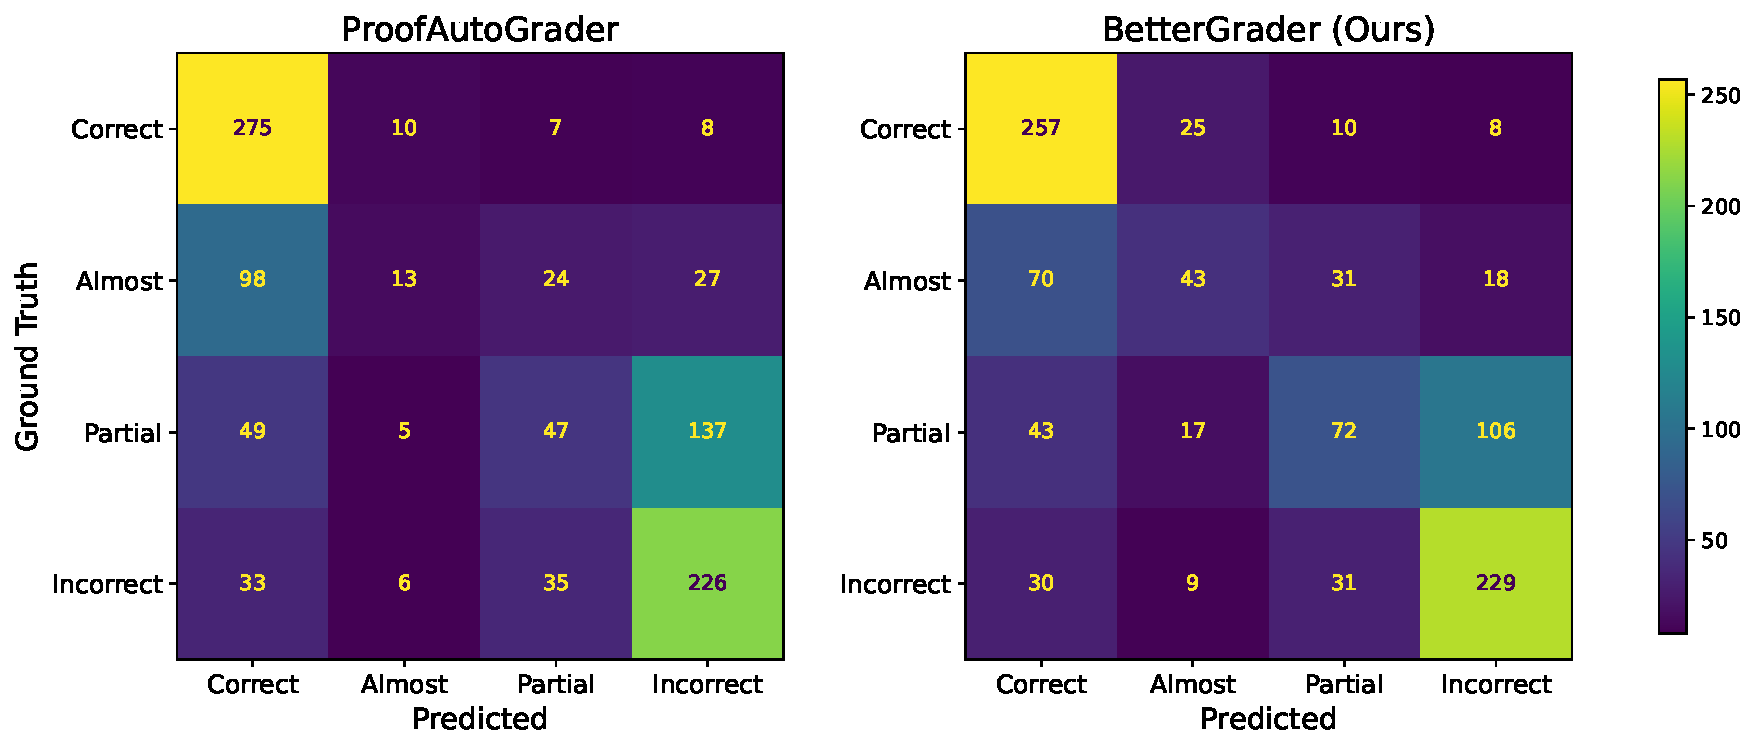
\includegraphics[width=\textwidth]{figures/ch_hyperagents/imograding_confmat.pdf}
\caption[Confusion matrices for IMO-level math graders]{\textbf{Confusion matrices for IMO-level math graders.} Comparison between (Left) ProofAutoGrader from \citet{luong2025towards} and (Right) BetterGrader discovered automatically by the DGM-H. BetterGrader reduces the collapse of intermediate solutions into extreme labels by correctly identifying more \textit{Almost} and \textit{Partial} cases, while maintaining strong performance on \textit{Correct} and \textit{Incorrect}. This shift toward better-calibrated intermediate judgments explains the gains in accuracy by BetterGrader.}
\label{fig:res-imograders}
\end{figure}

BetterGrader is produced automatically by the DGM-H without any domain-specific heuristics or handcrafted rules (Section~\ref{sec:results-compound}). BetterGrader's improvements over ProofAutoGrader \citep{luong2025towards} are driven primarily by correcting a grading bias that collapses nuanced solutions into extreme labels. The confusion matrices show that ProofAutoGrader frequently misclassifies intermediate cases as either \textit{Correct} or \textit{Incorrect}: for \textit{Almost}, it predicts \textit{Correct} 98 times (vs.\ 70 for BetterGrader) and \textit{Incorrect} 27 times (vs.\ 18), and for \textit{Partial} it over-assigns \textit{Incorrect} 137 times (vs.\ 106) (Figure~\ref{fig:res-imograders}). BetterGrader assigns intermediate labels more appropriately, substantially increasing true positives for \textit{Almost} (43 vs.\ 13) and \textit{Partial} (72 vs.\ 47), which matches the large gains in recall (\textit{Almost}: $+18.52\%$, \textit{Partial}: $+10.50\%$) and F1 (\textit{Almost}: $+0.203$, \textit{Partial}: $+0.109$). Although BetterGrader trades a modest decrease in \textit{Correct} recall ($-6.00\%$), a regime where ProofAutoGrader was already near-saturated at $91.67\%$, the net effect is higher overall accuracy ($+4.06\%$), consistent with a grader that better matches human granularity rather than defaulting to all-or-nothing judgments.

\subsection{Modifying Parent Selection}
\label{app:res-parentselect}

\begin{figure}[H]
\centering
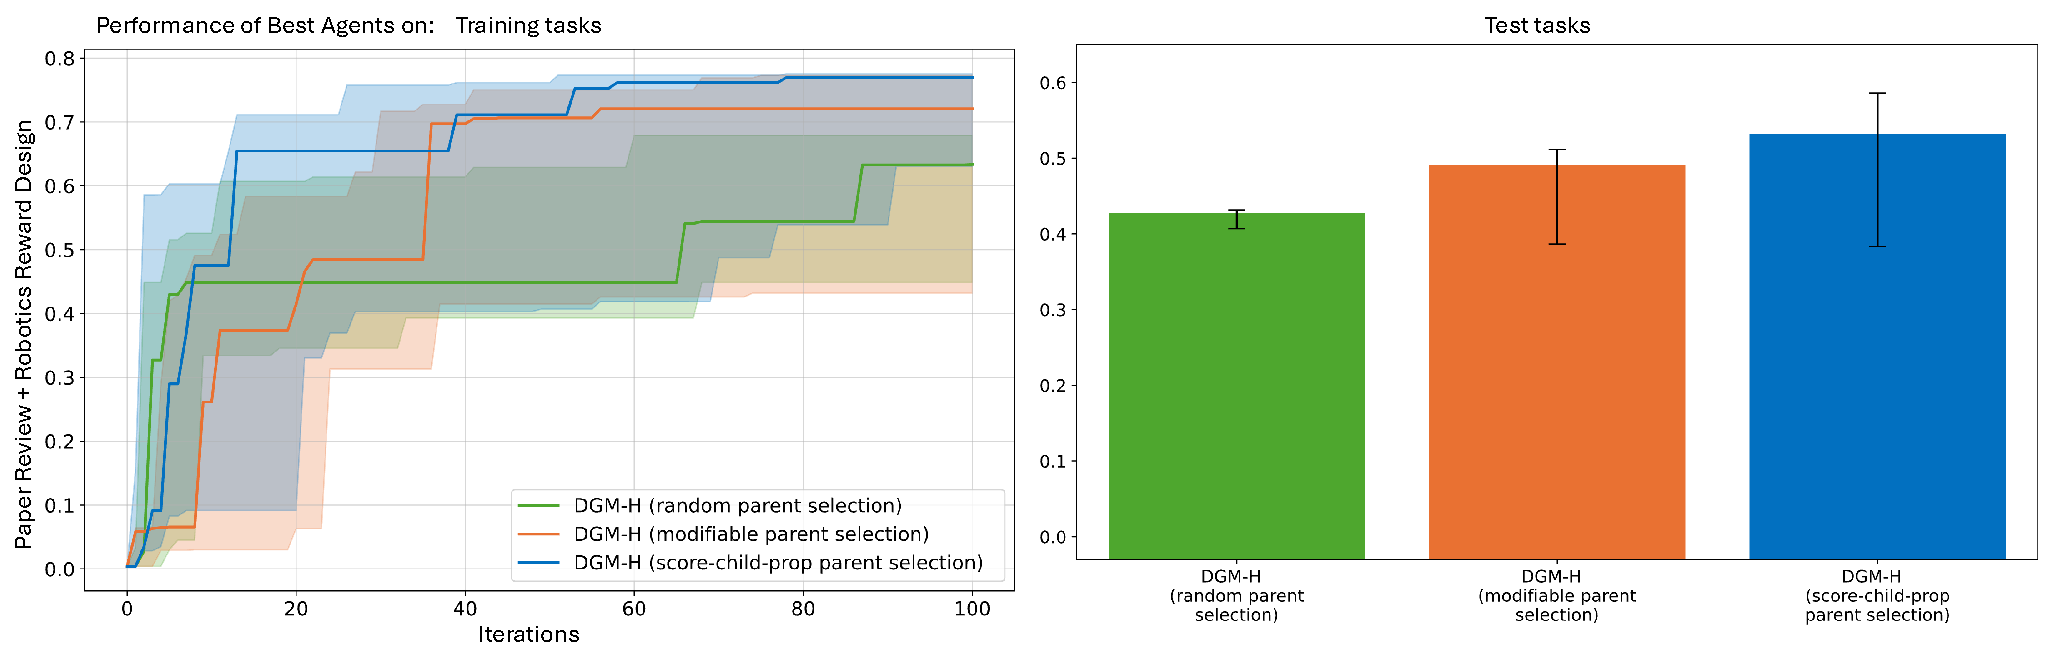
\includegraphics[width=\textwidth]{figures/ch_hyperagents/results_parentselect.pdf}
\caption[The DGM-H with modifiable parent selection mechanism]{\textbf{The DGM-H with modifiable parent selection mechanism.} (Left) The DGM-H improves the parent selection mechanism beyond random selection, but does not outperform a carefully handcrafted mechanism. (Right) The best agents discovered by each method are evaluated on test tasks in paper review and robotics reward design.}
\label{fig:res-parentselect}
\end{figure}

In this section, we investigate whether the DGM-H can automatically modify the parent selection mechanism. In all other experiments (Section~\ref{sec:results}), the DGM-H uses a fixed parent selection strategy that is roughly proportional to each agent's performance score and the number of its children that successfully compiled (\textbf{score-child-prop}) (Appendix~\ref{app:parent-selection}). In the DGM-H run with a modifiable parent selection mechanism (\textbf{modifiable}), we initialize the DGM-H with random parent selection and allow the agent to modify this mechanism over time (Algorithm~\ref{algo:DGM-H-parentselect}). We compare this setting against a baseline that uses random parent selection throughout the run (\textbf{random}). Each method is repeated across 5 repeated runs.

On test tasks, DGM-H with random parent selection improves average performance on paper review and robotics reward design from 0.030 (the initial agent) to 0.428 (CI: 0.407 -- 0.432). Allowing the DGM-H to modify the parent selection mechanism further improves performance to 0.491 (CI: 0.387 -- 0.512). The handcrafted score-child-prop parent selection achieves the highest performance, improving from 0.030 to 0.532 (CI: 0.384 -- 0.586). While these differences are not statistically significant ($p > 0.05$), they reveal a consistent qualitative trend: enabling meta-level modification of parent selection yields improvements over random selection, but does not yet surpass a carefully engineered mechanism (Figures~\ref{fig:res-parentselect},~\ref{fig:res-parentselect-archives}).

We qualitatively analyze how the DGM-H modifies the parent selection mechanism. Starting from random parent selection, the meta agent consistently replaces random sampling with structured exploration-exploitation strategies. Across all runs, the DGM-H independently creates variants of Upper Confidence Bound (UCB) \citep{auer2002finite} style selection, combining normalized performance with explicit exploration bonuses:

\begin{lstlisting}[language=Python]
exploration_bonus = exploration_weight * math.sqrt(
    math.log(total_children + 1) / (children + 1)
)
ucb_score = normalized_score + exploration_bonus
\end{lstlisting}

This pattern emerges within the first few iterations of every run, indicating that the meta-agent recognizes UCB-style selection as a broadly useful principle for open-ended search. Beyond UCB, the DGM-H evolves probabilistic selection mechanisms based on temperature-controlled softmax sampling:

\begin{lstlisting}[language=Python]
exp_scores = np.exp(scores / temperature)
probabilities = exp_scores / np.sum(exp_scores)
parent = np.random.choice(genids, p=probabilities)
\end{lstlisting}

Over time, the temperature parameter itself becomes adaptive, responding to archive size, recent progress, or stagnation. Later iterations further enhance parent selection with multi-component scoring systems that integrate additional signals such as diversity, recency, and elite performance. Several runs also introduce explicit stagnation detection, increasing exploration when progress slows:

\begin{lstlisting}[language=Python]
if score_variance < 0.01:
    exploration_weight *= 1.4
\end{lstlisting}

Despite the increasing sophistication, the automatically modified parent selection does not outperform a carefully handcrafted score-child-prop mechanism (Appendix~\ref{app:parent-selection}). Qualitatively, this appears to result from the added complexity and sensitivity of the learned mechanisms. Nonetheless, these results demonstrate that the DGM-H can autonomously recreate classic selection algorithms, extend them with adaptive heuristics, and explicitly reason about failure modes such as stagnation.

This is the pseudocode of DGM-H with modifiable parent selection:

\begin{algorithm}[H]
\DontPrintSemicolon
\SetAlgoLined
\KwIn{Initial agent $a^{0}$, task set $\mathcal{T}$, maximum iterations $T$}
\KwOut{Archive of scored agents $\mathcal{A}$}
\BlankLine
$s^{0} \leftarrow \textsc{Evaluate}(a^{0}, \mathcal{T})$\;
\textbf{initialize} $\mathcal{A} \leftarrow \{(a^{0}, s^{0})\}$\;

\For{$t \leftarrow 1$ \KwTo $T$}{
    $(a_{\text{latest}}, \cdot) \leftarrow \text{most recently added element of } \mathcal{A}$\;
    $\mathcal{P} \leftarrow a_{\text{latest}}.\textsc{SelectParents}(\mathcal{A})$ \tcp*{Parent selection by latest agent}
    \ForEach{$(a, \cdot) \in \mathcal{P}$}{
        $a' \leftarrow a.\textsc{Modify}(a, \mathcal{A})$ \tcp*{Metacognitive self-modification}
        $s' \leftarrow \textsc{Evaluate}(a', \mathcal{T})$\;
        \If{$\textsc{IsValid}(a')$}{
            $\mathcal{A} \leftarrow \mathcal{A} \cup \{(a', s')\}$\;
        }
    }
}
\Return{$\mathcal{A}$}
\caption{The DGM-H with modifiable parent selection}
\label{algo:DGM-H-parentselect}
\end{algorithm}

\begin{figure}[H]
\centering
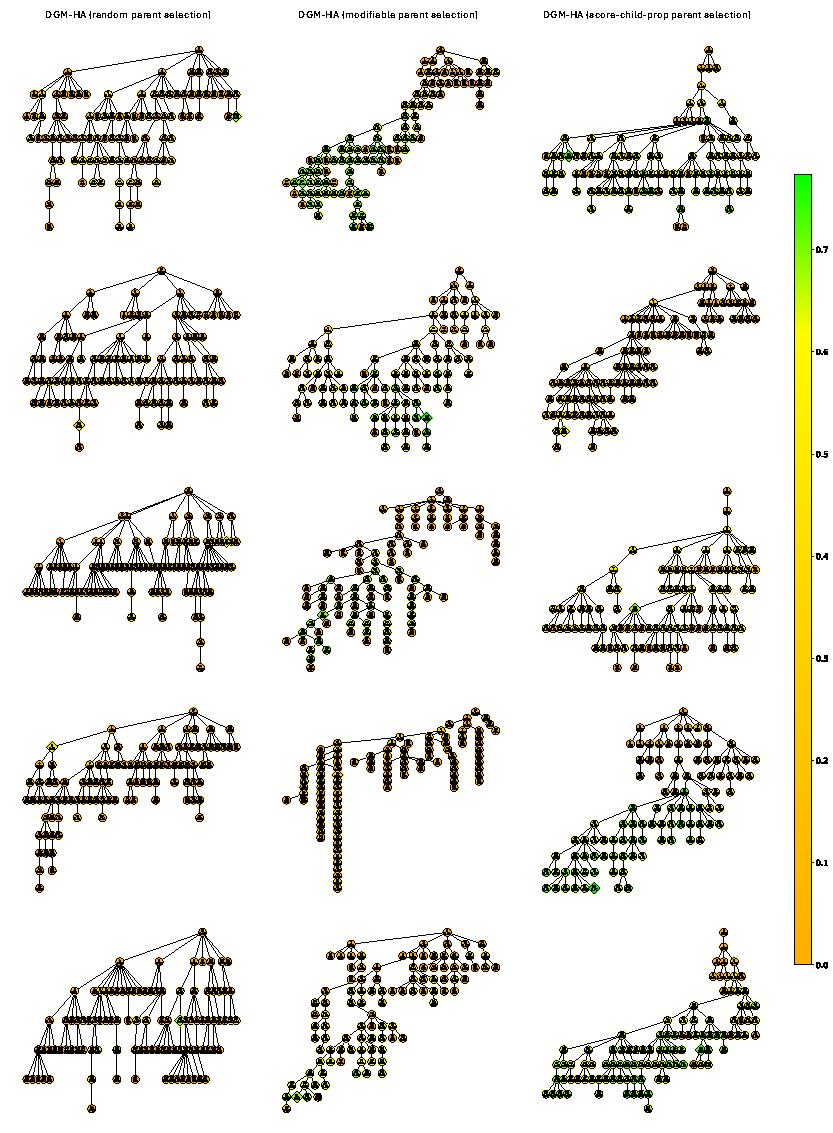
\includegraphics[width=0.9\textwidth]{figures/ch_hyperagents/results_parentselect_archives.pdf}
\caption[Archives generated under different parent selection strategies]{Archives generated under different parent selection strategies with DGM-H: (Left) random, (Middle) modifiable, and (Right) score-child-prop. Random parent selection generates many low-performing agents. Modifiable parent selection learns to balance exploration and exploitation, increasingly focusing on promising agents for branching. The carefully handcrafted score-child-prop parent selection consistently produces high-performing agents.}
\label{fig:res-parentselect-archives}
\end{figure}

\section{Safety Discussion}
\label{app:safety}

The DGM-Hyperagents (DGM-H) introduces distinct safety considerations due to its ability to autonomously modify its own behavior and improvement mechanisms over time. In this work, all experiments are conducted under strict safety constraints. In particular, agent-generated code is executed within carefully sandboxed environments with enforced resource limits (e.g., timeouts, restricted internet access). These measures are designed to prevent unintended side effects, contain failures, and ensure that self-modifications remain confined to the intended experimental scope. Moreover, evaluation is performed using predefined tasks and metrics, and human oversight is maintained throughout all experiments.

\textbf{Potential to evolve faster than human oversight.}
As AI systems gain the ability to modify themselves in increasingly open-ended ways, they can potentially evolve far more rapidly than humans can audit or interpret. At the cusp of such explosive capability growth, it becomes necessary to reconsider the roles that AI systems play in society \citep{bengio2024managing}. Rather than framing safety solely in terms of absolute guarantees or full interpretability, a central challenge lies in balancing the potential of AI as a catalyst for human progress and well-being (e.g., automating scientific discovery) with the degree of trust humans are willing to place in these systems \citep{clune2019ai, ecoffet2020open, bengio2024managing, weston2025ai}.

\textbf{Reflection and amplification of human biases.}
In this work, objectives are specified through fixed benchmarks and evaluation criteria. The DGM-H does not alter the underlying task definitions; instead, it optimizes performance with respect to the provided objectives. As a result, the DGM-H reflects the norms and biases present in the data and benchmarks on which it is trained. In this sense, the system acts both as a clarifier and an amplifier of existing human behavior. This underscores the importance of careful benchmark design, dataset curation, and periodic re-evaluation of evaluation criteria.

\textbf{Evaluation gaming.}
Another safety concern arises from the risk of evaluation gaming, a manifestation of Goodhart's law \citep{strathern1997improving}, where optimizing for a metric leads to improvements on the metric without progress on the intended underlying objective. Because the DGM-H optimizes empirical evaluation signals, self-improving agents may discover strategies that exploit weaknesses or blind spots in the evaluation procedure. Mitigating evaluation gaming requires robust, diverse, and periodically refreshed evaluation protocols, as well as complementary metrics, held-out tests, and human oversight.

While the DGM-H operates within safe research boundaries (e.g., sandboxing, controlled evaluations), these safeguards may become increasingly strained or infeasible as self-improving systems grow more capable. We proactively include this discussion to encourage broader engagement with what safety means for open-ended self-improving AI systems \citep{clune2019ai, ecoffet2020open, sheth2025safety}.
